% \begin{appendix}
\section{Fotodokumentation - Zwei Semester Anfängerpraktikum}
% \centering
% \begin{figure}
% \includepdf[width=0.9\textwidth, pages={1}]{Bilder/Messdaten.pdf}
% \end{figure}
% \newpage
% \begin{figure}
% \includepdf[width=0.9\textwidth, pages={2}]{Bilder/Messdaten.pdf}
% \end{figure}
%
% \end{appendix}

\begin{figure}
  \centering
  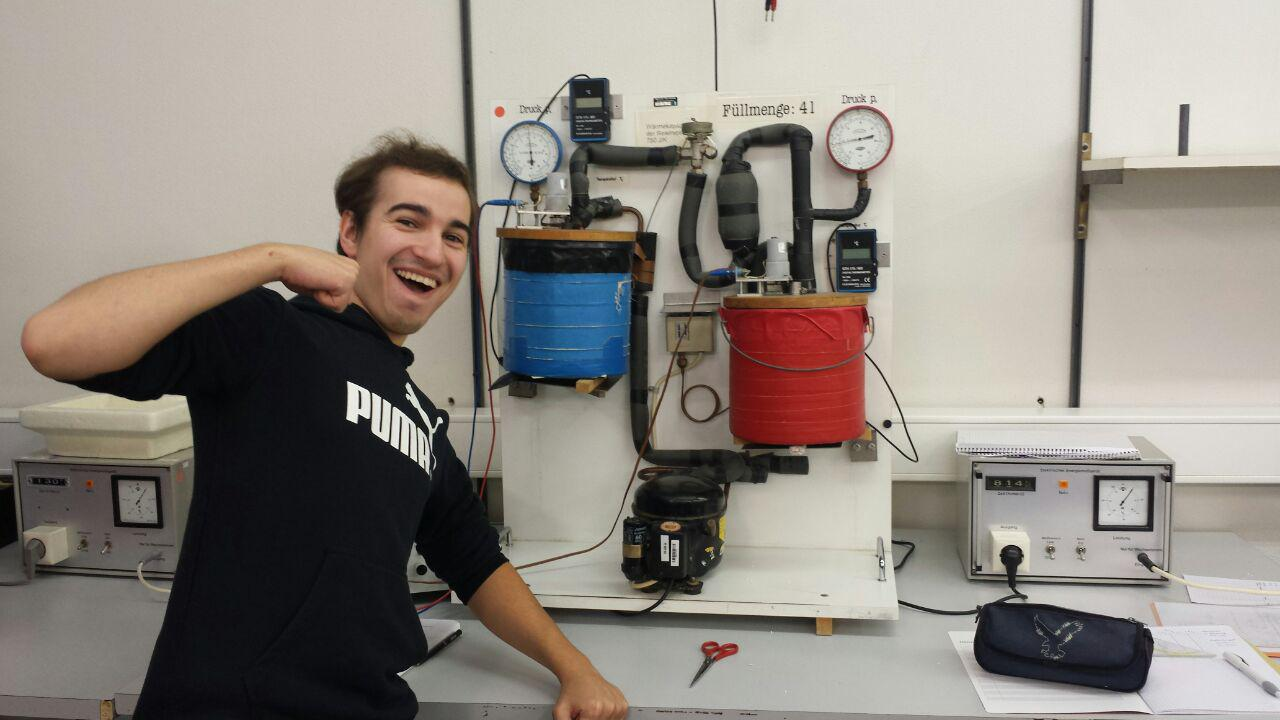
\includegraphics[height=5cm]{extra/photo_2016-07-05_00-27-30.jpg}
  \caption{Der erste Versuch - Mit voller Motivation an die Wärmepumpe!}
\end{figure}

\begin{figure}
  \centering
  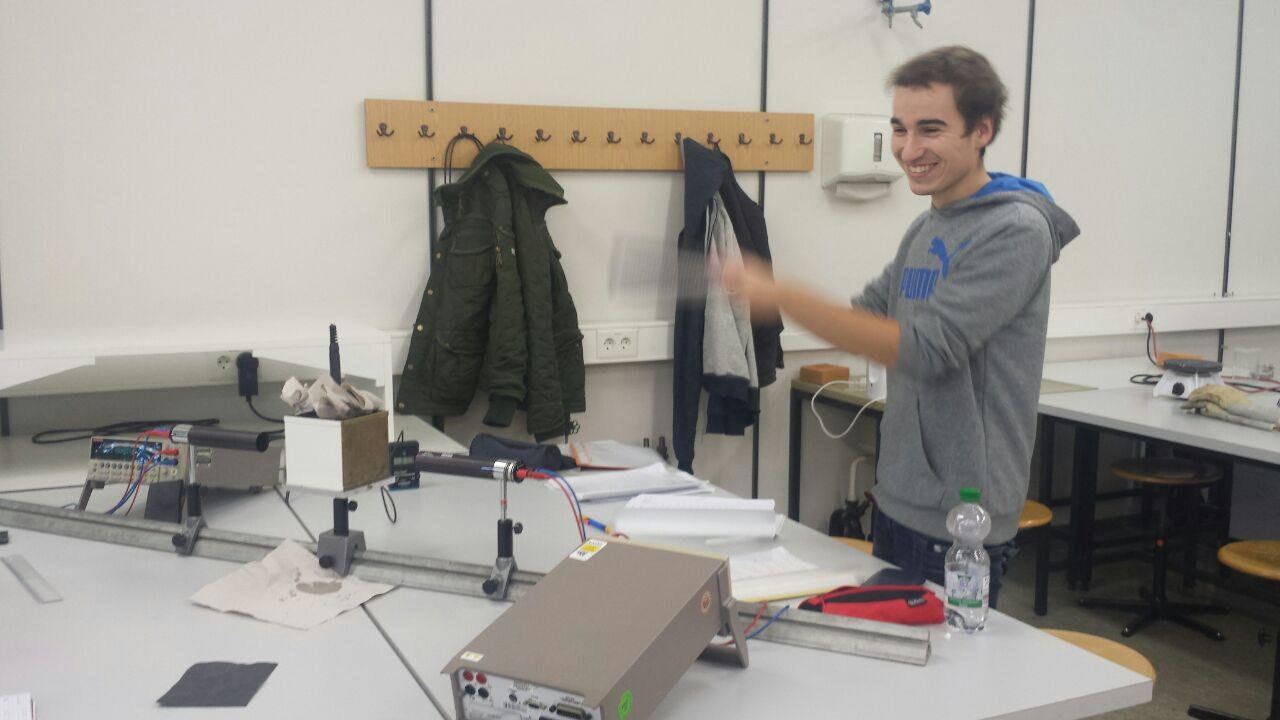
\includegraphics[height=5cm]{extra/photo_2016-07-05_00-36-25.jpg}
  \caption{Professionelle Kühlungsverfahren beim Leslie-Würfel.}
\end{figure}

\begin{figure}
  \centering
  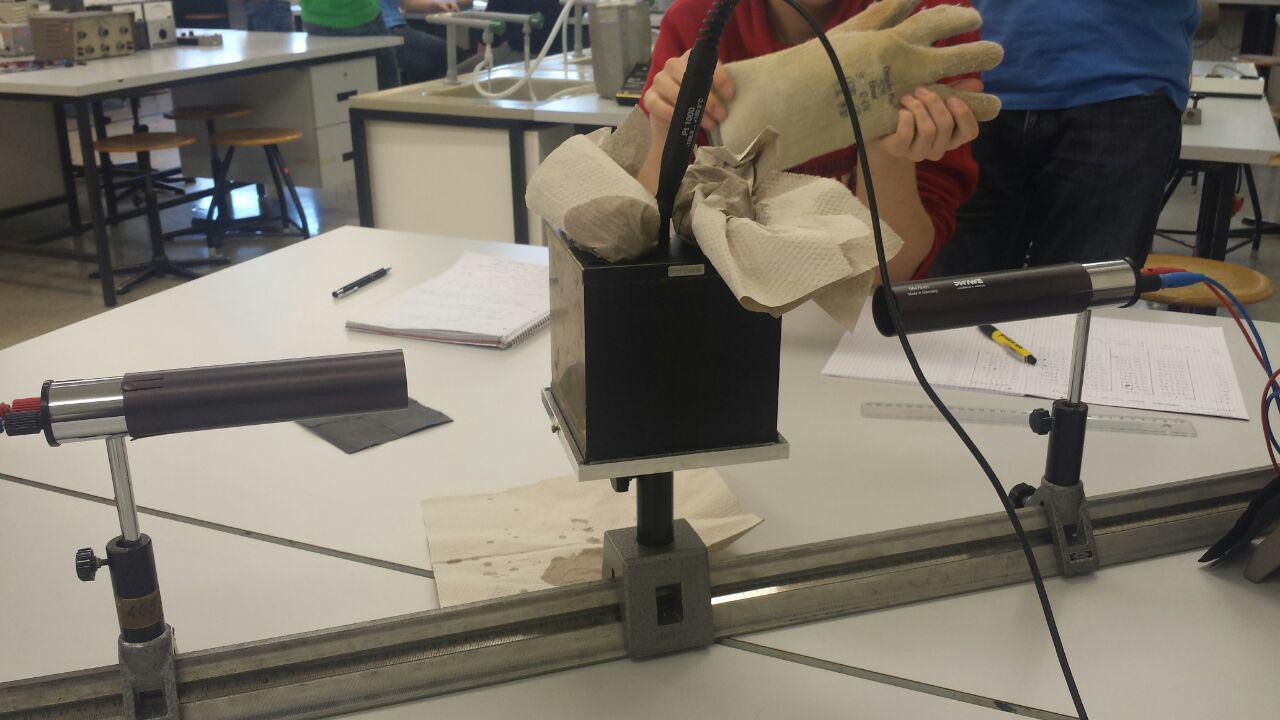
\includegraphics[height=5cm]{extra/photo_2016-07-05_00-38-18.jpg}
  \caption{Professionelle Kühlungsverfahren beim Leslie-Würfel.}
\end{figure}

\begin{figure}
  \centering
  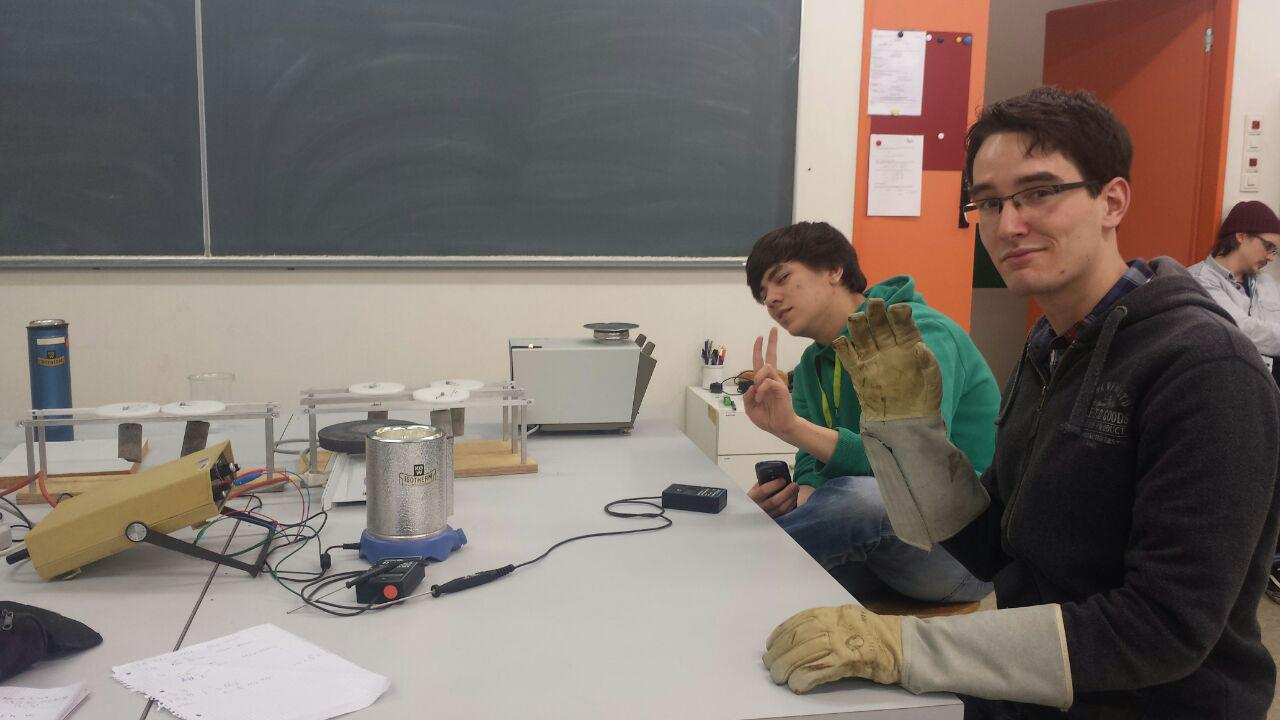
\includegraphics[height=5cm]{extra/photo_2016-07-05_00-37-24.jpg}
  \caption{Unsere ständigen Begleiter - Hier beim Dulong-Petite Gesetz. Der erste Versuch, bei dem wir komplett verzweifelt sind...}
\end{figure}

\begin{figure}
  \centering
  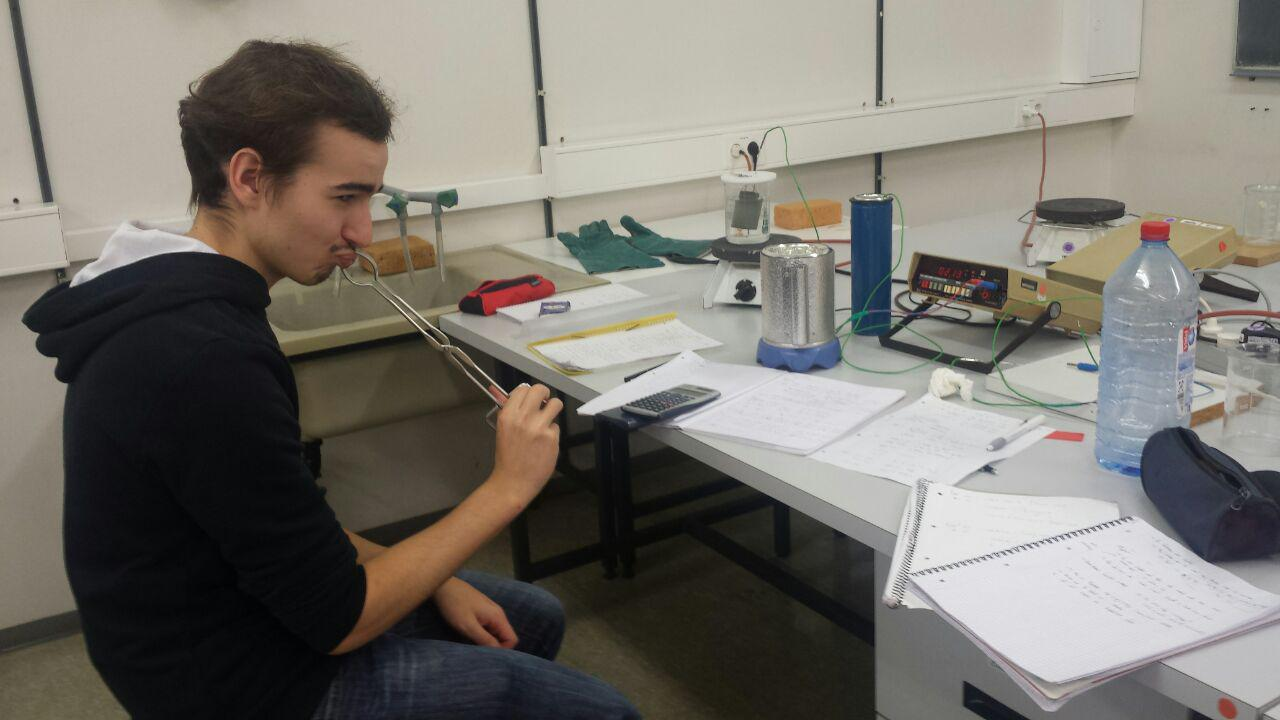
\includegraphics[height=5cm]{extra/photo_2016-07-05_00-39-07.jpg}
  \caption{... aber am Ende ist doch alles gut ausgegangen.}
\end{figure}

\begin{figure}
  \centering
  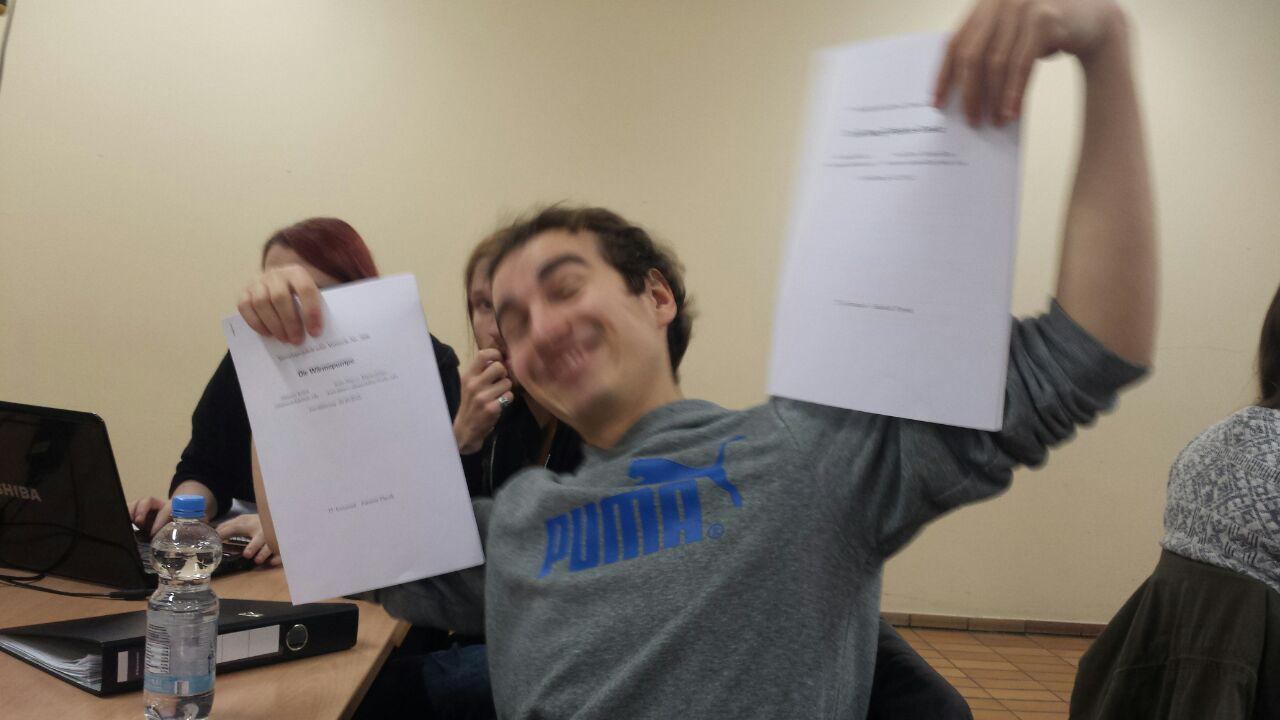
\includegraphics[height=5cm]{extra/photo_2016-07-05_00-39-29.jpg}
  \caption{Voller Stolz: Die ersten Abgaben!}
\end{figure}

\begin{figure}
  \centering
  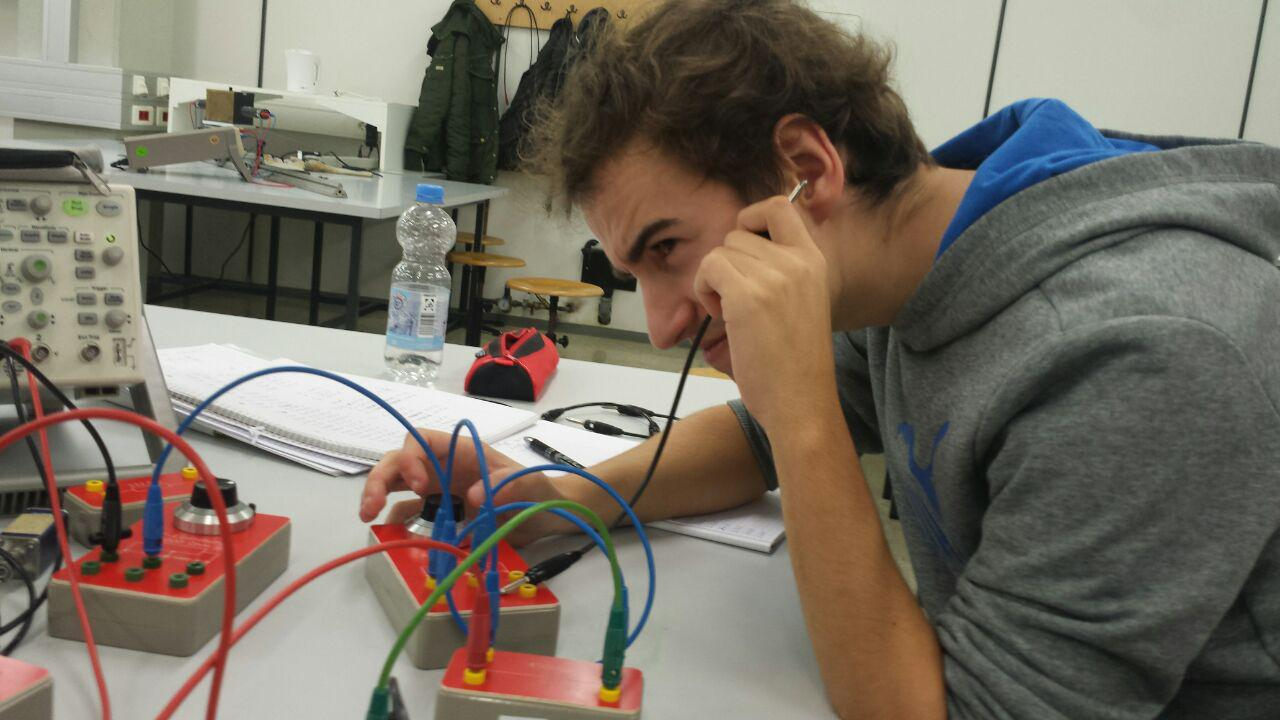
\includegraphics[height=5cm]{extra/photo_2016-07-05_00-40-34.jpg}
  \caption{Auch das korrekte Messen von Spannungen will gelernt sein.}
\end{figure}

\begin{figure}
  \centering
  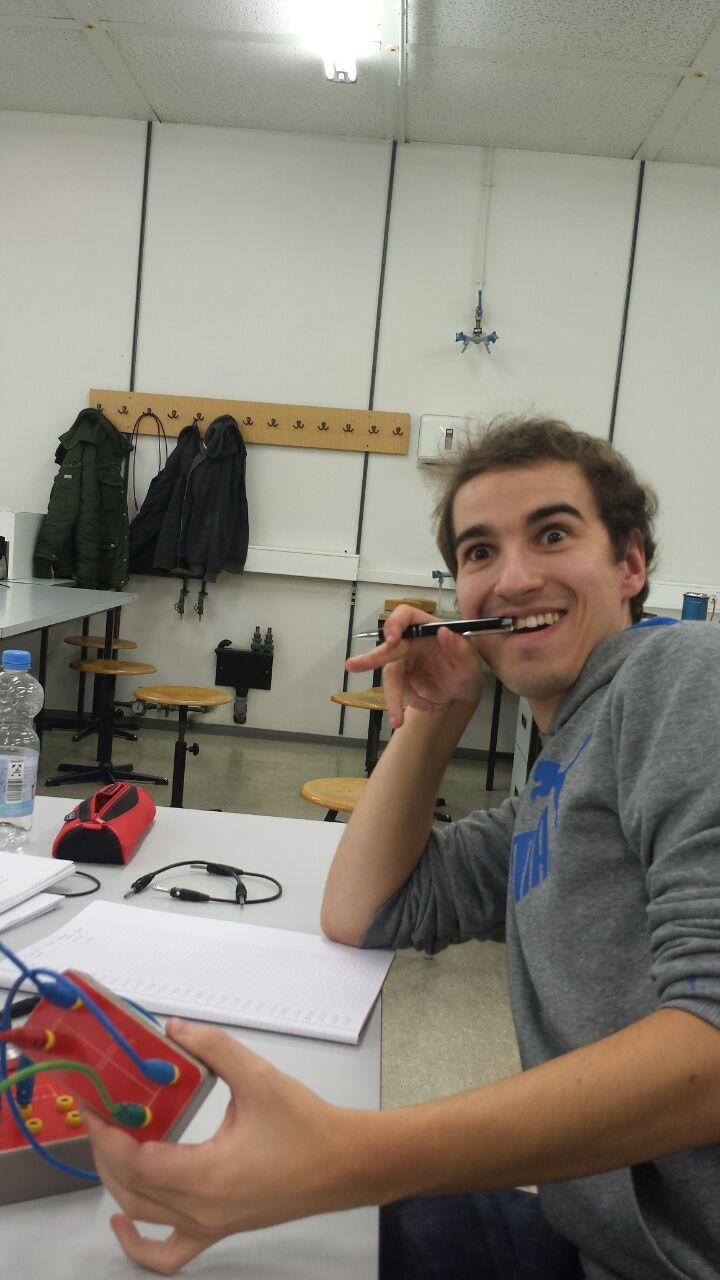
\includegraphics[height=5cm]{extra/photo_2016-07-05_00-44-22.jpg}
  \caption{Auch das korrekte Messen von Spannungen will gelernt sein.}
\end{figure}

\begin{figure}
  \centering
  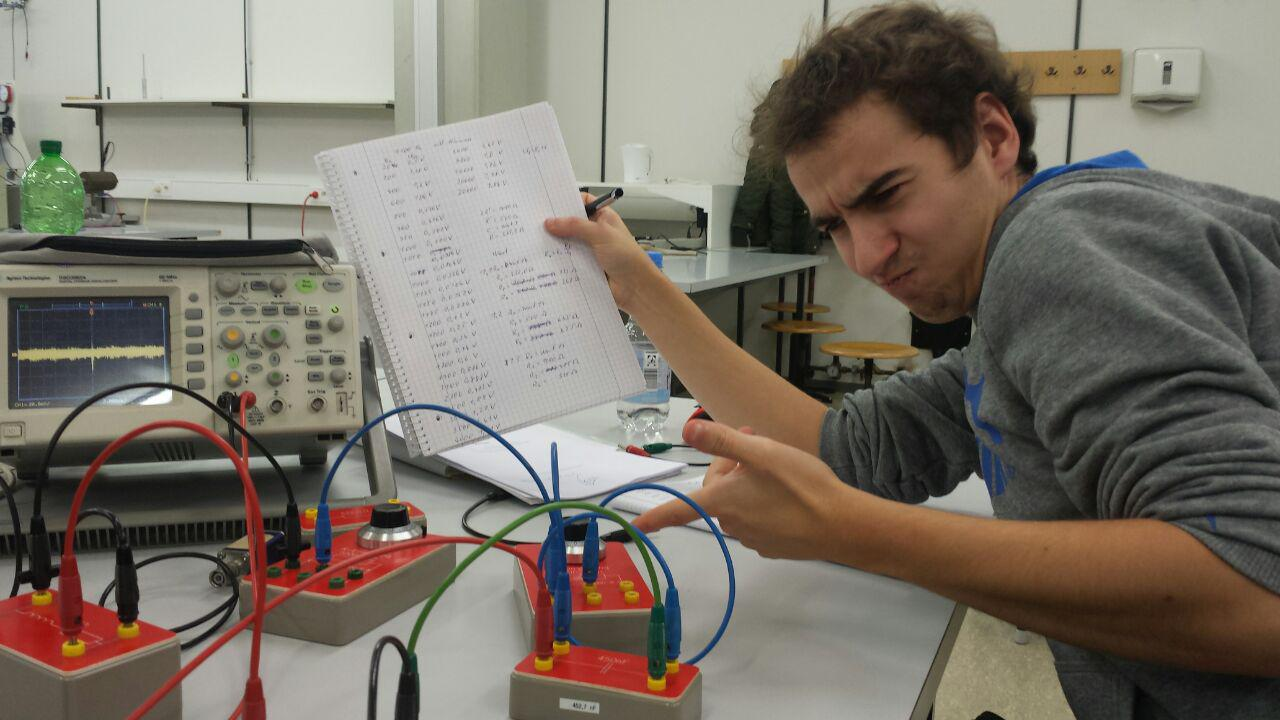
\includegraphics[height=5cm]{extra/photo_2016-07-05_00-41-15.jpg}
  \caption{Und auch wenn mal nicht sofort was geklappt hat bei den Elektronikversuchen: Der Brückenschaltungsmann war immer zur Stelle.}
\end{figure}

\begin{figure}
  \centering
  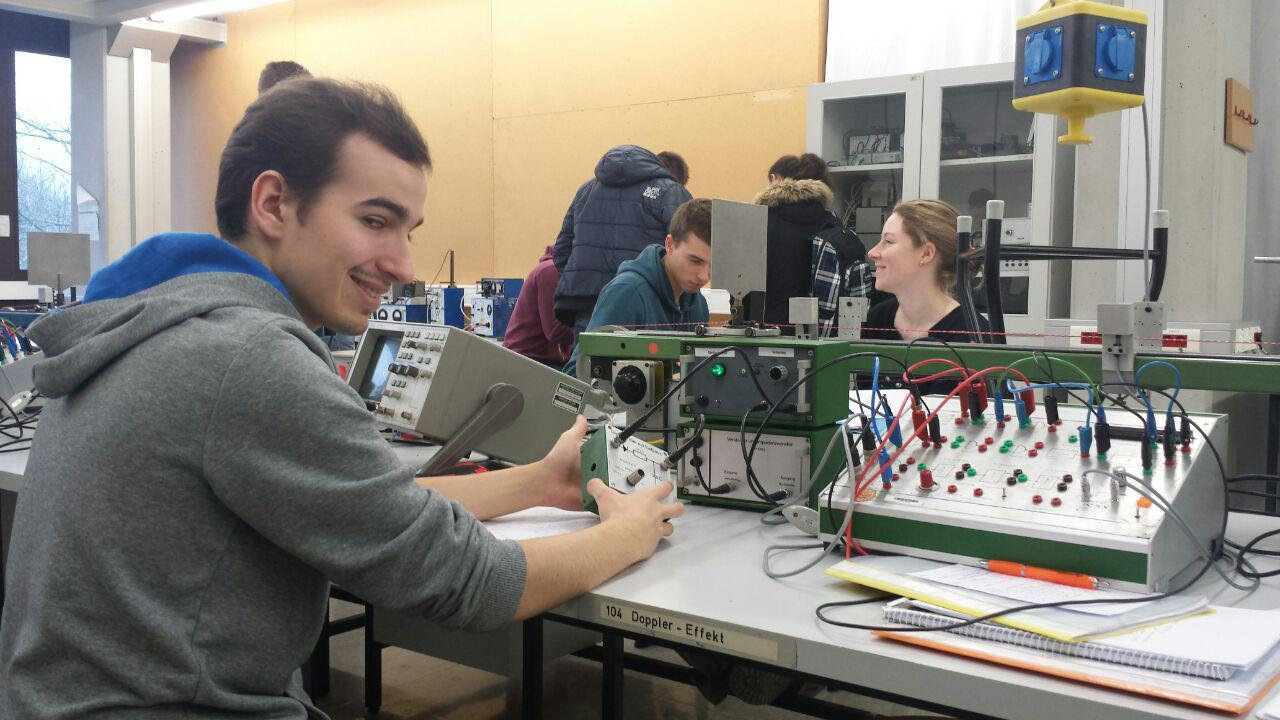
\includegraphics[height=5cm]{extra/photo_2016-07-05_00-41-59.jpg}
  \caption{Der Gleichrichter und Tiefpass beim Doppler-Effekt.}
\end{figure}

\begin{figure}
  \centering
  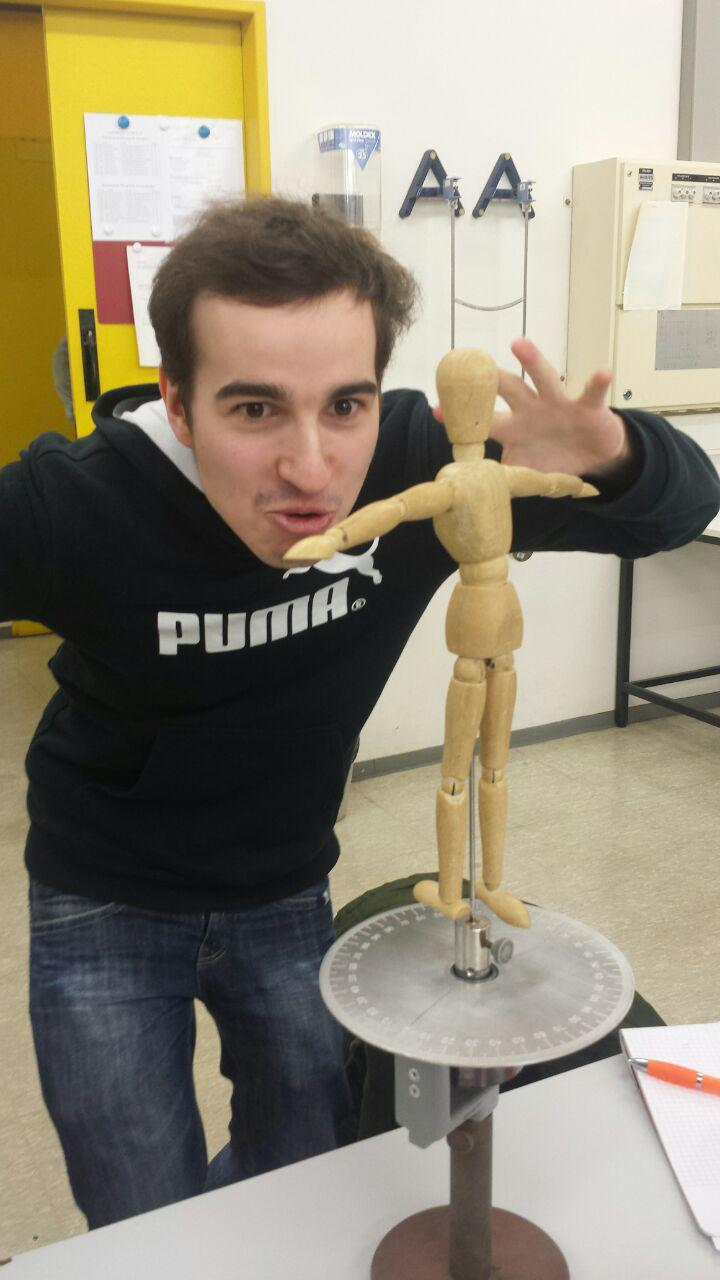
\includegraphics[height=5cm]{extra/photo_2016-07-05_00-44-49.jpg}
  \caption{Professionelle Dokumentation der Puppen bei den Trägheitsmomenten.}
\end{figure}

\begin{figure}
  \centering
  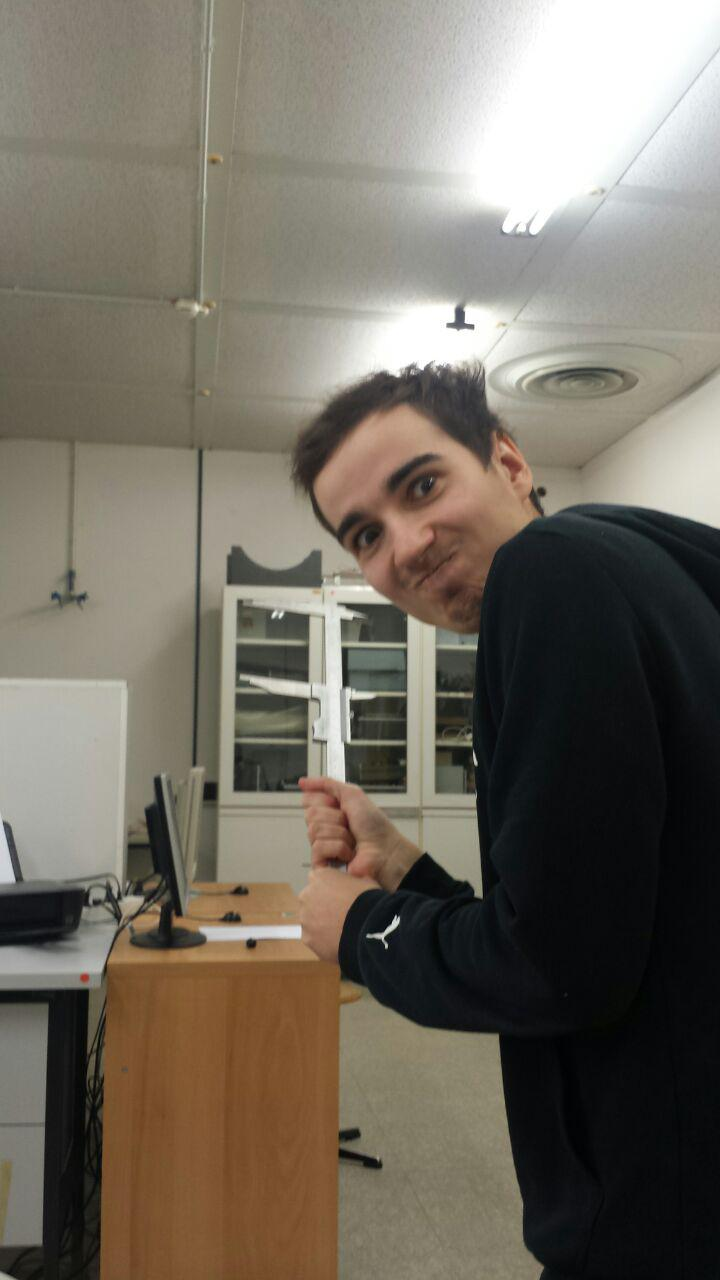
\includegraphics[height=5cm]{extra/photo_2016-07-05_00-46-06.jpg}
  \caption{Professionelles Vermessen der Puppen bei den Trägheitsmomenten.}
\end{figure}

\begin{figure}
  \centering
  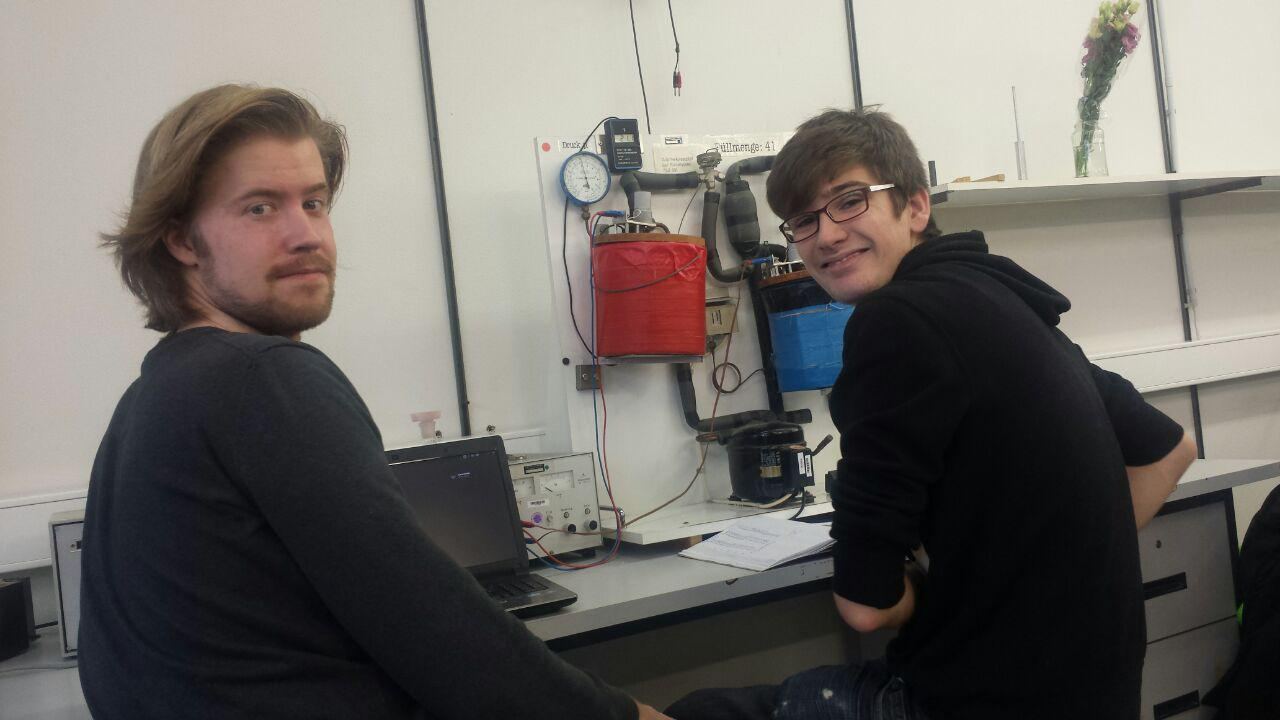
\includegraphics[height=5cm]{extra/photo_2016-07-05_00-45-21.jpg}
  \caption{Ebenfalls treue Begleiter: Das Praktikumsduo AP-MaMa in Form von Marius und Matthias.}
\end{figure}

\begin{figure}
  \centering
  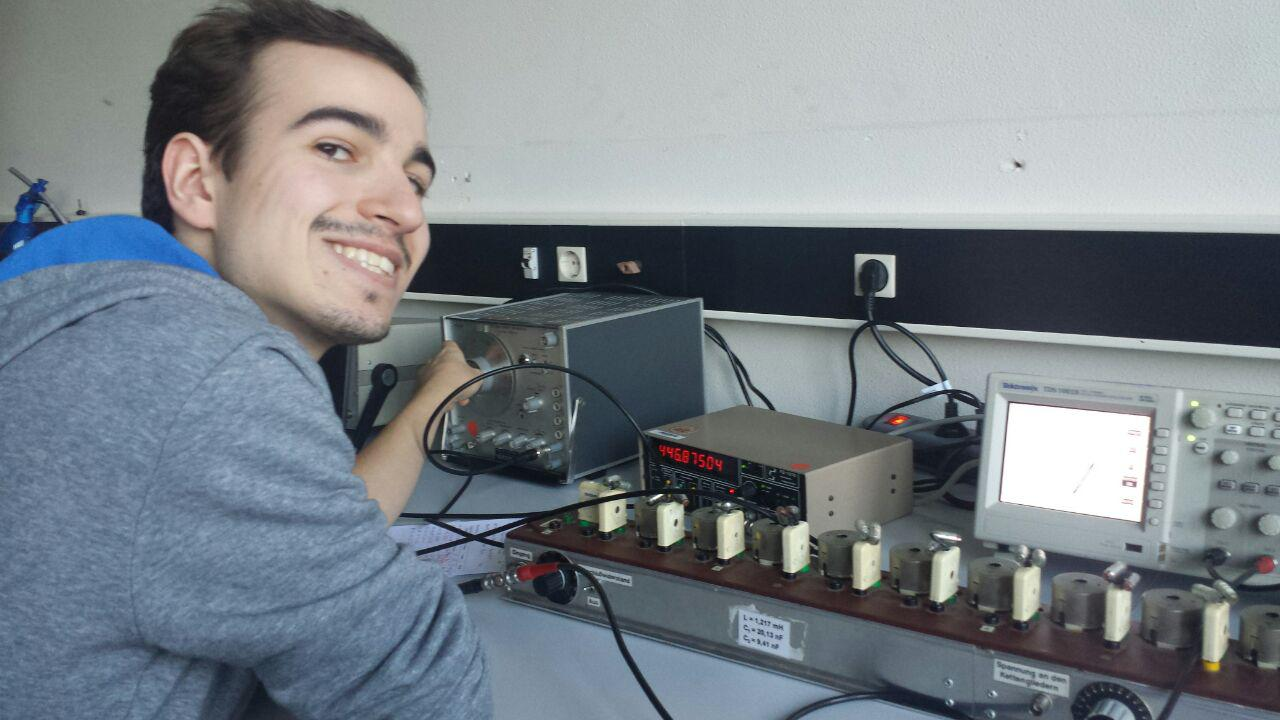
\includegraphics[height=5cm]{extra/photo_2016-07-05_00-47-04.jpg}
  \caption{Und natürlich der legendäre Ebberg-Raum mit V355 und V356!}
\end{figure}

\begin{figure}
  \centering
  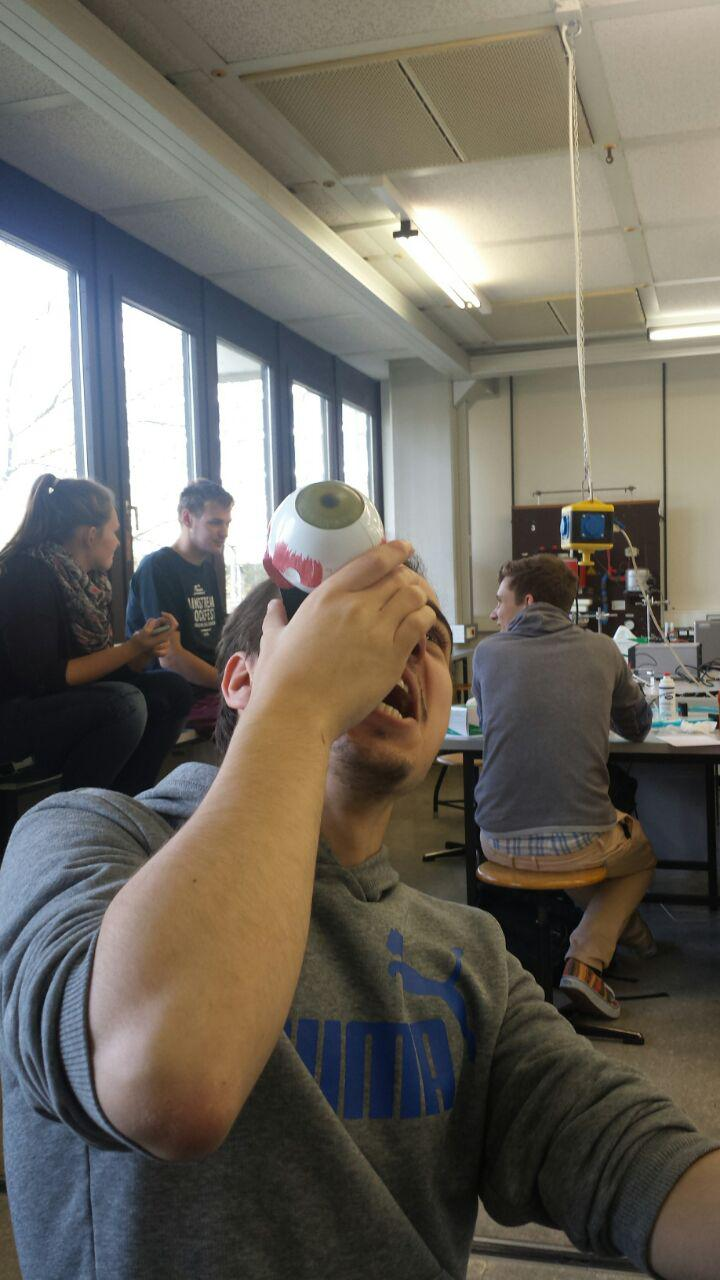
\includegraphics[height=5cm]{extra/photo_2016-07-05_00-48-00.jpg}
  \caption{Ahhhhhhhhh! Ultraschall!}
\end{figure}

\begin{figure}
  \centering
  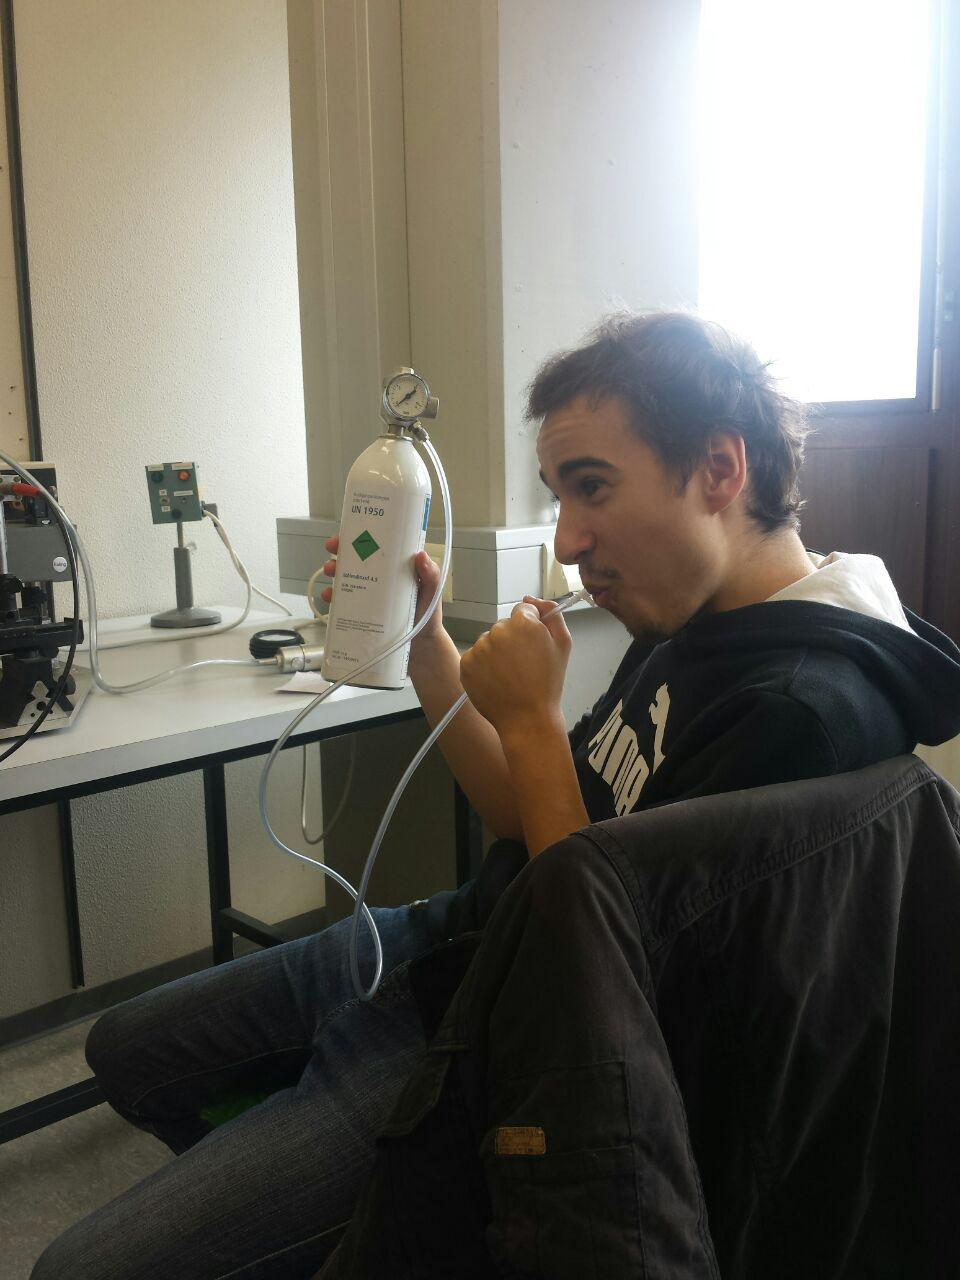
\includegraphics[height=5cm]{extra/photo_2016-07-05_00-48-33.jpg}
  \caption{Geschmacksprobe der verwendeten Gase beim Michelson Interferrometer!}
\end{figure}

\begin{figure}
  \centering
  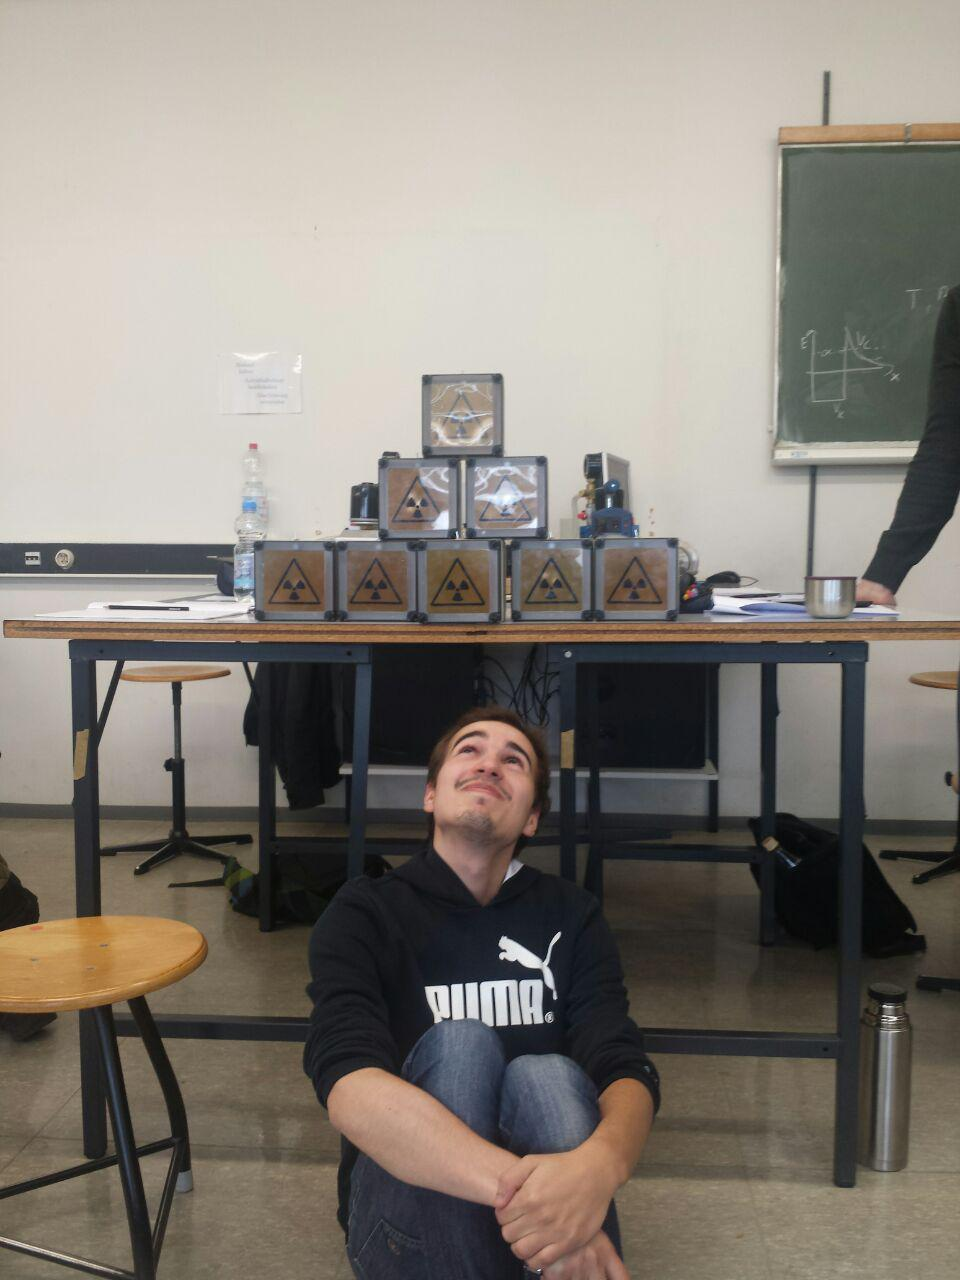
\includegraphics[height=5cm]{extra/photo_2016-07-05_00-49-08.jpg}
  \caption{Safety first bei den Kernversuchen.}
\end{figure}

\begin{figure}
  \centering
  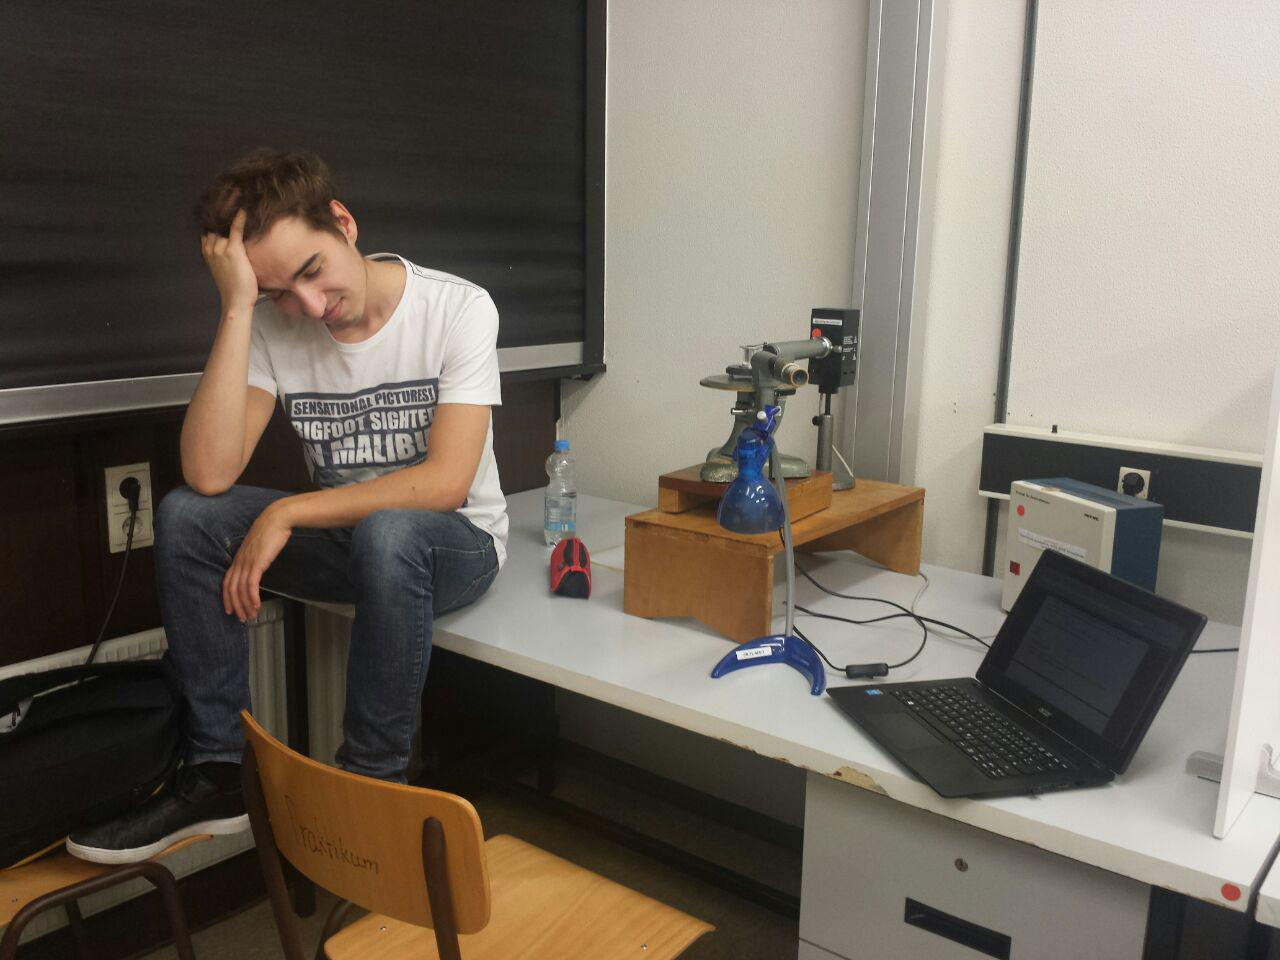
\includegraphics[height=5cm]{extra/photo_2016-07-05_00-49-57.jpg}
  \caption{Pure Verzweiflung bei den Dispersionsmessungen...}
\end{figure}

\begin{figure}
  \centering
  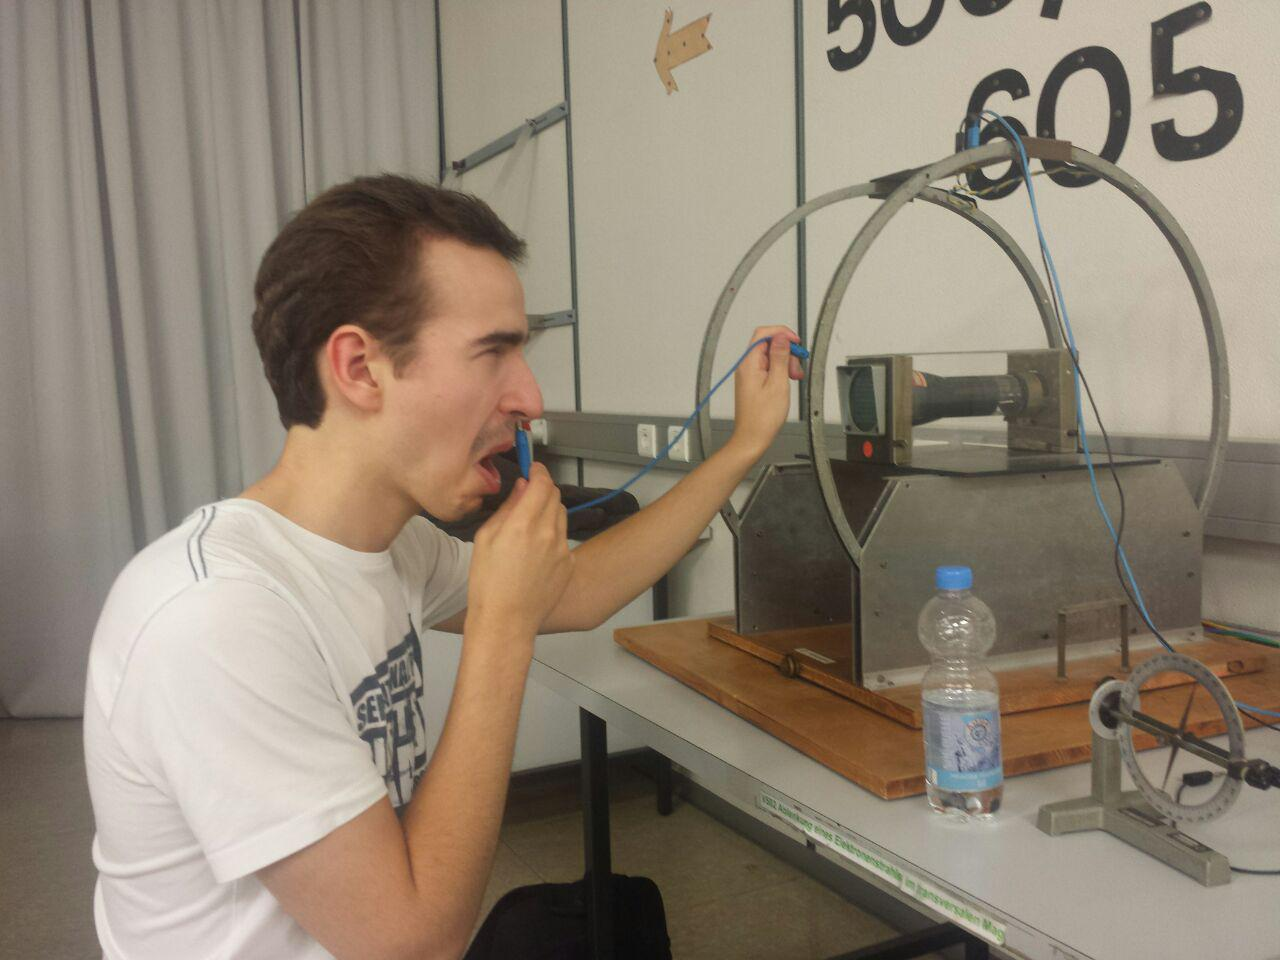
\includegraphics[height=5cm]{extra/photo_2016-07-05_00-50-37.jpg}
  \caption{Messen von Stromstärken: Gelernt im dritten Semester.}
\end{figure}

\section{Nachwort}
So schnell gehen zwei Semster Anfängerpraktikum um.
Nach meinem schnellen Versprechen, die Versuche möglichst umfangreich zu Dokumentieren und am Ende in einer Fotocollage zusammenzufassen, wurde dies nun in die Tat umgesetzt.
Zu sagen bleibt noch ein großer Dank meinerseits an meinen Praktikumspartner Johannes.
Auf dich war immer Verlass, auch wenn ich selber mal verhindert war oder weniger Zeit hatte.
Zudem war das Praktikum niemals langweilig, wie man gut an den Fotos sehen konnte!
Vielen Dank!

\textit{Jean-Marco Alameddine}
